\documentclass[12pt]{article}
\usepackage[utf8]{inputenc}
\usepackage{graphicx}
\usepackage{amsmath}
\usepackage{cite}
\title{
	{
\includegraphics[scale=0.3]{university.png}}\\
	{\large Amirkabir University of Technology}\\
	{Simulation report on my selected paper entitled "Energy Cost Optimization in Dynamic Placement
of Virtualized Network Function Chains"}\\
	}
\author{ Ali Zamani}
\date{16 July 2018}

\begin{document}


\maketitle

\newpage

\tableofcontents

\newpage

\section{Introduction}
The energy crisis has been a significant issue for years, as most resources are non-renewable such as oil, coal, and gas.The majority of the world’s energy comes from non-renewable resources, which, due to the large amounts of greenhouse gases emitted (such as carbon dioxide), lead to global warming.To add to this concern,energy consumption and greenhouse gas emissions resulting from Internet usage have been steadily increasing in recent years. For example, data center web servers, such as those used by Google and Facebook, account for 2\% of the greenhouse gas emissions  about the same as air travel.

Fortunately, virtualization technology can spur a -------
ogy has a
very high migration cost both in terms of time and energy.
 Most importantly, its management is only limited to the
service provider. 

we can minimize
energy consumption using NFV technology, which can extend
virtualization to other PMs, such as routers, switches, etc.
Physical machines consume maximum power only during
peak demand times, and average servers remain idle over 90\%
of the time. However, the power consumption of an idle
machine is nearly 60\% of the peak load power consum ption of
the machine [18]. By reducing the number of active machines,
and turning off the idle machines, we can reduce the energy
consumption of the network.

we use the minimum capacity mechanism
 to minimize the frequent change of the machines’ states.
According to this mechanism, we required a minimum
capacity to transit an OFF node to an ACTIVE node. This
helps to increase the utilization of the machine. Fifty percent
of the power consumed by the PMs is to reduce heat generated
during proce ssing . Hence, depending on the PM load, the
cooling load also varies . Therefore, in this paper, we
normalize the energy consumption cost of the PMs, and the
respective VM instances on those machines, which will help
with performing a better analysis of the network’s energy
consumption issues. We consider the dynamic service chain
placement, which is a more realistic scenario than static
placement. However, in this work, we do not consider the
energy consumption of the link, as the difference of  the energy
consumption of the link from idle to full utilization is very
minimal.

novel contribution is summarized as follows:
1) First, we design an energy-saving model using an
M/M/c queuing network
for the placement of multiple service chains’
functions in the network.
2) We formulate an optimization problem to minimize
the total energy consumption cost of the network
with capacity and delay as the constraints and prove
that NP-hard.
3) We propose an efficient dynamic placement of VNF ains (DPVC) heuristic algorithm for the dynamic
placement of VNFs in the network. Via MATLAB
experimentation, we demonstrate that our algorithm
significantly minimizes the cost of energy
consumption.

\subsection{Network Function Virtualization}
Network Function Virtualization (NFV)  technology has emerged as a new alternative, which can overcome the pitfalls. NFV offers a new way to design,deploy , and manage networking services by decoupling the network functions, such as network address translation,firewalls, intrusion detection, domain name service, etc., from dedicated hardware devices so they can run in software. These network functions are called virtualized network functions (VNFs), and they are placed on physical machines as virtual machine (VM) instances.ftware provisioning. An example of service chain placement
in the network is presented in Figure 1. The network consists
of nine nodes considered as the physical machines of the
network. We have four different network functions: $ A, B, C,
D,$ which are available in different nodes of the network, as
shown in Figure 1.Tabel 1 shows four service chain demands,
with the source and destination paths of four different flows.
The virtual links and physical path of each flow from source to
destination are  given in the table. The first service chain, $SC1$
$(B–C–A)$, at source node $1$, will be placed in the sequence of
nodes $2, 4, 7$. That is, the first VNF $B$ will be placed on node
$2$, then the second VNF$C$ will be placed on node $4$, where
the function $C$ is available. The final VNF of $SC1$ will be
placed on node $7$ and the chain will terminate at destination
node $6$. Similarly, the second service chain, $SC2$$ (C–A–D)$,will start from source node $5$, terminate at destination node $
ch 1$,
and place VNFs on nodes $9, 7, 4$. The third service chain, $SC3$
$(A–D–B)$, will start from source node $6$, terminate at
destination node $1$, and place VNFs on nodes $7,4, 2$.
However, for the fourth service chain, $SC4 (B–D–B)$, from the
source node $5$, after placement of the first VNF$B$ on node $9$,
the next function $D$ is not available in the neighboring nodes.
Therefore, it will be placed on node$ 4$, the last VNF$B$ will
be placed on node $2$, and finally, it will terminate at 
destination node $6$. 

\begin{figure}[t!] \label{fig:1}
  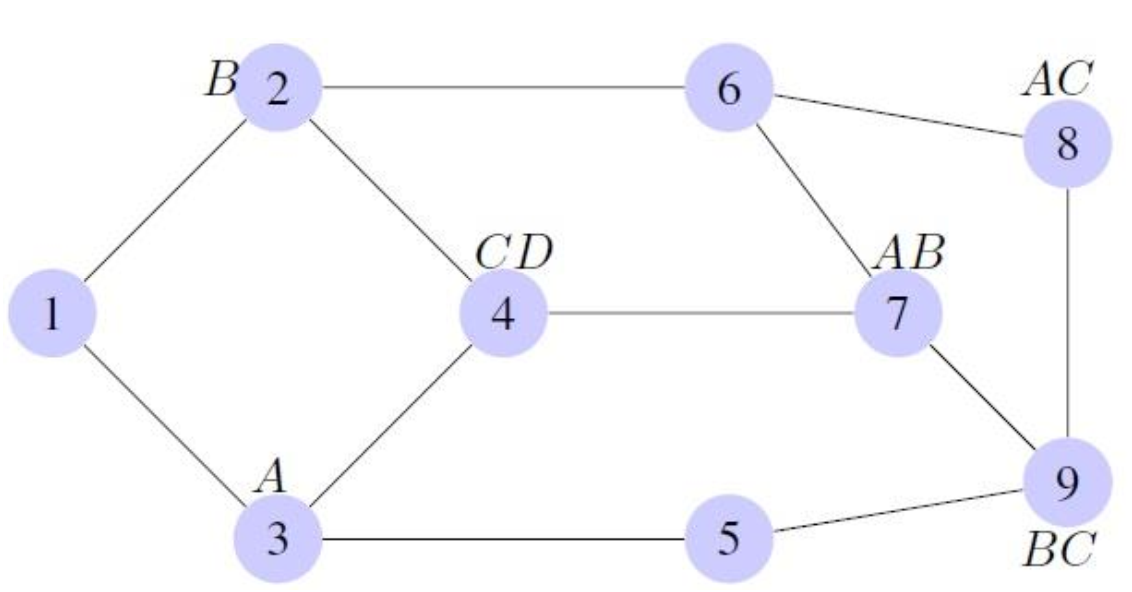
\includegraphics[width=\linewidth]{fig1.png}
  \caption{ Illustrative example of service chain placement in the network.}
\end{figure}

\begin{table}[t!]
\caption{VNF placement of the service chains.}

\centering
\begin{tabular}{|c|c|c|c|c|c|} 
 \hline
 SC number& Source&Destination&SC Demand&Virtual Path&Physical Path \\ [0.5ex] 
 \hline 
SC1&1&6&B-C-A&1-2-4-7-6&1-2-4-7-6 \\ [0.5ex]  
 \hline
SC2&5&1&C-A-D&5-9-7-4-1&5-9-7-4-2-1 \\ [0.5ex]
 \hline
SC3&6&1&A-D-B&6-7-4-2-1&6-7-4-2-1 \\ [0.5ex]
 \hline
SC4&5&6&B-D-B&5-9-4-2-6&5-9-7-4-2-6 \\ [1ex]
 \hline
\end{tabular}
\label{table:1}
\end{table}

\section{Design and modeling}
\subsection{Off-Idle-Active State Transitionel}
Figure 2 illustrates the Off-Idle-Active (OIA) state transition
diagram of the PM. Each machine has three states named ---
nsumption of the machine can be evaluated in each state as
well.

(1) OFF$\rightarrow$ACT: Initially, the machine is in an OFF state,
and it consumes zero power$(Zpower)$. The machine will turn
ACTIVE when the sum of the capacities of the VNFs in the
queue exceeds the minimum capacity, or when the waiting
time of any VNF in the queue exceeds the maximum waiting
time. We adopted this method to maximize utilization and to
avoid the machine from engaging in the switching state too
often. This method 
also minimizes the waiting time of the
VNFs, which were waiting in the queue for a longer time.

(2) ACT$\rightarrow$IDL:When all VNFs in the ACTIVE machine
finish or migrate to other machines, the machine will go to the
IDLE state. In the IDLE state, a machine will consume the
basic amount of energy, which can be evaluated as the product
of maximum power $(Mpower)$ consumed by the machine and
the ratio between default capacity$(Dcap)$ of the machine to
the maximum capacity $(Mcap)$ of that machine
.

(3)IDL$\rightarrow$OFF: If no new VNFs are assigned to the
machine in the IDLE state within a predefined time, the
machine will turn OFF.

(4)IDL$\rightarrow$ACT: If new VNFs are assigned, or if the VNFs
migrate from other ACTIVE machines, the machine will turn
ACTIVE from the IDLE state. Evaluation of the machine’s
energy consumption in the ACTIVE state is similar to the
IDLE state, only we need to add the summation of the
capacities of the deployed VNFs $(\sum Vcap)$ in the machine to
the  default capacity of the machine. Here, the maximum
power of the machine represents the maximum computing and
cooling power of the machine.
\subsection{M/M/c Queuing Network Model}
Many analytical models have been presented by various
articles using the M/M/1 queuing model.
However, in practice, real-world applications are not
processed by the single-service node. Therefore, we use the
M/M/c queuing network model , where each service
chain request can be processed through multiple service nodes,
a nd each service node can process multiple network functions.
Our energy-saving model adheres to the following
assumptions. The VNFs of the service chain arrivals follow a
Poisson process  and are served in the order of their arrivals
i.e., the $(i+ 1)$th VNF of a service chain can start only after
completion of the $i$th VNF of that service chain. In our model,
a service node can process a maximum $c$  number of VNFs of
different service chains together. We assume all service chains
are independent. All service times are independent and
exponentially distributed with mean $1/\mu$. The idle time follows
the exponential distribution with mean: $1/\theta_1$, and the off time
follows exponential distribution with mean: $1/\theta_2$. Both
aforementioned variables are independent of each other. Here,
the state space is settled by $S=\{(m, n), m = \{0,1\}, 0 \preceq n \preceq \inf \}$
, where $m$ denotes the machine is ON or OFF, and $n$ denotes
the number of VNFs in the machine. The state-transition-rate
diagram for a queuing system is shown in Figure 3. State (0, 0)
denotes that the machine is ON, but with no VNF, i.e., the
IDLE state, and $(0, n)$ denotes that the machine is ACTIVE
with $n$ number of VNFs. State $(1, n)$ shows the OFF state with
$n$ number of VNFs in waiting.

Let $P_{m,n}$
denote the steady-state probabilities at state $(m,n)$,
then the following notations are used:

$P_{0,n}$= Probability that $n$ VNFs exist in the PM in the
ACTIVE state.

$P_{0,0}$ = Probability that  no VNFs exist in the PM, and it is
IDLE.

$P_{1,n}$= Probability that $n$ VNFs exist in the PM in the OFF
state.

Based on Figure 3, the following balanced equations can be
given:
\begin{equation}
(\lambda+\theta_1)P_{0,0}=\mu\sum_{n=1}^{c}n.P_{0,n}
\end{equation}
\begin{equation}
(\lambda+c\mu)P_{0,n}=\lambda.P_{0,n-1}+c\mu.P_{0,n+c}\quad      where( n=1,...,c-1)
\end{equation}
\begin{equation}
(\lambda+c\mu)P_{0,n}=\lambda.P_{0,n-1}+c\mu.P_{0,n+c}+\theta_2.P_{1n}\quad      where( n=c,c+1,...,\infty)
\end{equation}
\begin{equation}
\theta_1.P_{0,0}=\lambda.P_{1,0}
\end{equation}
\begin{equation}
\lambda.P_{1,n}=\lambda.P_{1,n-1} \quad where (n=1,...,c-1)
\end{equation}
\begin{equation}
(\lambda+\theta_2)P_{1,n}=\lambda.P_{1,n-1} \quad where (n=c,c+1,...,\infty)
\end{equation}
Let $P_{ACTIVE}$, $P_{IDLE}$,and $P_{OFF}$ denote the probabilities that a
PM is in the ACTIVE, IDLE, and OFF states respectively.
With the normalizing equation $\sum_{n=1}^{\infty}P_{0,n}+P_{0,0}+\sum_{n=0} ^{\infty}P_{1,n}=1$
, the solutions of these equations can be obtained as:
\[ 
  \begin{cases}
    P_{ACTIVE}=\sum_{n=1}^{\infty}P_{0,n}\\
    P_{IDLE}=P_{0,0}\\
    p_{OFF}=\sum_{n=0}^{\infty}P_{1,n}
  \end{cases}
\]

$Theorem 1:P_{OFF}=\sum_{n=0}^{\infty}P_{1,n}=[c.\frac{\theta_1}{\lambda}+\frac{\theta_1}{\theta_2}]P_{0,0}$.
Assuming, $\alpha =\frac{(\theta_1+\lambda).k.(k+c)}{2c^2} $  
 for some large integer$k$, we have,\\

$Theorem 2:P_{ACTIVE}=\sum_{n=1}^{\infty}P_{0,n}=[\frac{\alpha}{c\mu}+\frac{\theta_1}{\lambda+c\mu}]$.\\

$Theorem 3: if \sum_{n=0}^{\infty}P_{0,n}+\sum_{n=0}^{\infty}P_{1,n}=1, then P_{0,0}=\frac{1}{1+\frac{\theta_1}{\theta_2}+\frac{c\theta_1}{\lambda}+\frac{\alpha}{c\mu}+\frac{\theta_1}{\lambda+c\mu}}$\\

By using this value $P_{0,0}$ we can find $P_{OFF},P_{IDLE}$ , and
$P_{ACTIVE}$ of each PM. That is, we can determine what is the
state of the machine, and how many VNFs are on the machine.
Then, as given in Figure 2, the amount of the power consumed
by the machine in different states can be evaluated
\begin{figure}[!t] \label{fig:2}
  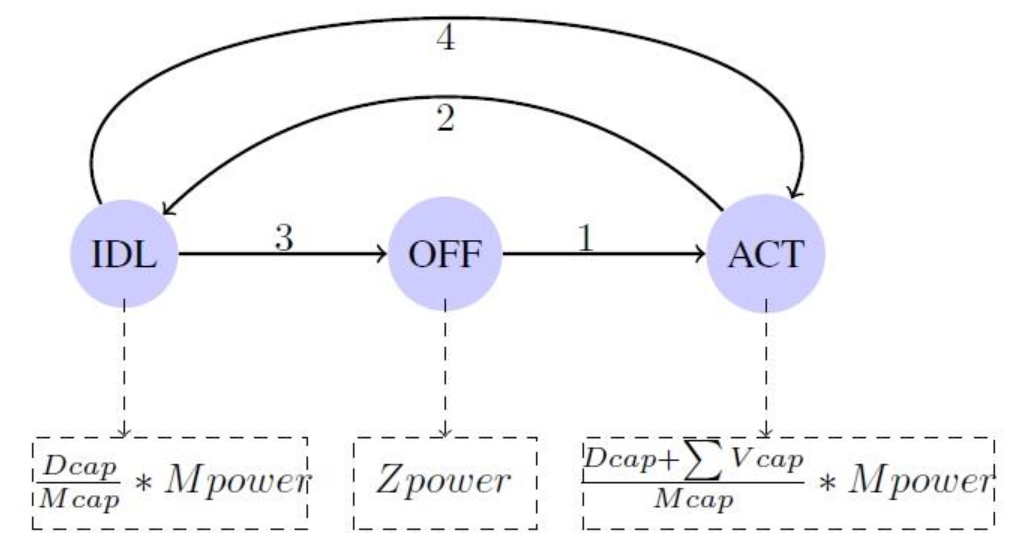
\includegraphics[width=\linewidth]{fig2.png}
  \caption{OIA state transition diagram of PM}
\end{figure}
\begin{figure}[!t] \label{fig:3}
  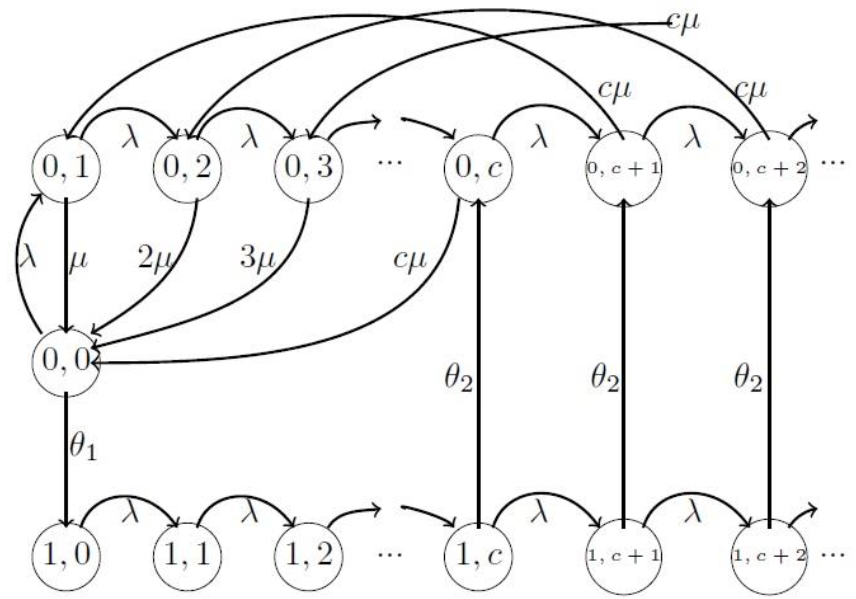
\includegraphics[width=\linewidth]{fig3.png}
  \caption{M/M/c queuing model state transition diagram for a service node.}
\end{figure}
\section{Problem Formulation}

 we can get the state of
a PM at a particular time and the number of VM instances on
the PM at that time. Considering this, we propose an
optimization problem to minimize the energy consumption
cost in this section.
\subsection{Variable Declaration}
In Table 2, we declared the variables used to formulate the
optimization problems. We classify all variables in four
groups. The first group represents the different sets we will
use. $N$ and  $L$ are the set of nodes and links, respectively.
Here, a node means a PM. $sC$ represents the set of all
requested service chains and $vF$ is the set of VNFs we have in
our network.$T$  is the set of iterations.$vM$  is the set of VM
instances on a particular node and $K$ is the set of commodities.

The second group represents the variables and different
network parameters we will use. $n(u)$ is the decision variable
of the physical machine $u$, which shows the state of the
machine. $s_k$ and $t_k$ are the source and destination of
commodity $k$, respectively. $F_k$ is the flow of commodity $k$,
and $P_k$ is the path of flow $k$. $e_u^N$ shows the energy consumed
by the node $u$. $e_c$ and $te_c$ are the energy consumption cost and
the total energy consumption cost, respectively. 

The third
group refers to the delay, demand, and capacity parameters.
$C^N(u), C^I(u), and$  $C_i^v(u)$ represent the maximum capacity,
default capacity, and capacity of the VM instance $i$ of the node
$u$, respectively. $C^L(u,v)$ is the capacity of link $(u,v)$ and
$d_k(u,v)$ is the delay faced by the flow $k$ at link $(u,v)$.
$qd_f^{sc}(u)$ is the queuing delay of the function $f$ of service
chain $sc$ at node $u.d_{MAX}(u)$  is the maximum delay at node $u$,
and $D_k$ is the maximum delay that the flow can tolerate.
$d_f^{sc}(u)$ represents the demand of function $f$ of service chain $sc$
at node $u$. The last group consists of two binary variables.
$X_i^f(u)$ presents function $f$ placed on the $i$th VM instance of
node $u$.$Y_f^{sc}(u)$ shows the function $f$ of service chain $sc$
placed on node $u$.

\begin{table}[t!]
\caption{List of commonly used variables and notations}
  \includegraphics[width=\linewidth]{fig4.png}
\centering
\label{table:2}
\end{table}

\subsection{Objective Function and Constraints}

By using the notations given in Table 2, we state the
energy consumption cost is:
\begin{equation}
e_c=\sum_{u\in\omega}n(u)*(\frac{c^I(u)+\sum_{i\in{vM(u)}}C_i^v(u)}{C^N(u)})
\end{equation}

$where \quad n(u)=
			\begin{cases}
				1,if\  node(u) \ is\  IDLE\  or\  ACTIVE\\
				0,otherwize
			\end{cases}
$	
\\
The total energy consumption cost $te_c=\sum_{t\in{T}}e_c(t)$. Here,
$n(u)$ represents the state of the node $u$. The value is 1 if the
node is ACTIVE or IDLE, and 0 otherwise.$C^N(u)$,$C^I(u)$,
and $C_i^v(u)$ represent the maximum capacity, default capacity
of the machine in the IDLE state, and capacity of the VM
instance $i$ (on $u$ ) of the node $u$, respectively. $e_u^N$ is the cost of
energy consumed by node $u$ at a utilization of 100\%. $e_c(t)$ is
the cost of energy consumption by the network at time $t$. The
total cost of energy  consumption $te_c$ of the network is the sum
of energy consumption of each individual node in various
states over a period of time. Our objective is to $Minimize \quad te_c$. The set of operational constraints to be
noticed are:		
\\
$1)$ $Flow Constraints:$The inequality in Equation (8) ensures
that the flow from node $u$ to node $v$ must be positive.
Equation (9), ensures that the total flow along each link should
not exceed the total capacity of that link. The flow
conservation constraint is sh own in Equation (10), where $r_k$
unit of traffic is created in its source, and is destroyed in its
destination. For a stable system, the limit of the utilization of
each node and links lies between [0 , 1]. Equation (11) ensures
the utilization limit of each PM.
\begin{equation}
F_i(u,v)\geq 0 ,\quad , \forall i , \ F_i \in K,\forall (u,v) \in L
\end{equation}


\begin{equation}
\sum_{i=1}^k F_i(u,v) \leq C^L(u,v)*L(u,v),\quad \forall (u,v) \in L
\end{equation}

\begin{equation}
\sum_{(u,v)\in L}F_k(u,v)-\sum_{(v,u)}F_k(v,u)=\begin{cases}
								r_k,\ if \ u=s_k\\
								-r_k,\ if u=t_k
								0,\ otherwise
								\end{cases}
\end{equation}


\begin{equation}
0  \leq \frac{\lambda}{c\mu} \leq 1
\end{equation}
$2)Capacity Constraints:$The inequality in Equation (12)
ensures that the total sum of the capacities of VNFs on node $u$
must be less than or equal to ‘utility capacity’ of node $u$, i.e.,
the difference between maximum capacity and default
capacity of $u$. The variable in Equation (13) shows the
function $f$ of service chain $sc$ is placed on node $u$. The
Equation (14) inequality ensures that the demand of function $f$
of service chain $sc$ at node $u$ must be less than or equal to the
available capacity of node $u$. The next inequality in Equation
(15) presents the demand of function $f$ of service chain $sc$ at
node $u$ less than or equal to the capacity of the VM instance $i$
of the node $u$.

\begin{equation}
\sum_{i \in vM(u)} C_i^V(u) \leq C^N(u)-C^I(u),\quad \forall (u) \in N
\end{equation}

\begin{equation}
Y_F^{sc}(u) =1,\quad \forall (u) \in N,f \in vF,\ sc \in sC
\end{equation}

\begin{equation}
\sum_{sc \in sC} d_f^{sc}(u) \leq C^N(u)-\sum_{i \in vM(u)} C_i^V(u)-C^I(u),\quad \forall (u) \in N,\ f \in vF,\ sc \in sC
\end{equation}

\begin{equation}
d_f^{sc}(u)\leq C_i^V(u),\quad \forall (u) \in N,\ f \in vF,\ sc \in sC
\end{equation}
$3) Placement Constraints:$The binary variable in Equation
(16) shows the function $f$ placed on the $i$th VM instance of
node $u$. The inequality in Equation (17) shows the queuing
delay of function $f$ of service chain $sc$ must be less than or
equal to the maximum delay at node $u$. Equation (18) ensures
that the delay faced by a flow along its path must be less than
or equal to the maximum delay the flow can tolerate. Equation
(19) checks the status of the node for the placement of the
function. It consists of three parts. The first inequality checks
whether the node is ACTIVE or not, and the  second part
checks the node is IDLE or not. The last part checks if the
node is OFF or not, and whether the demand on the node
exceeds the threshold value.

\begin{equation}
X_i^f(u)=1,\quad \forall (u) \in N
\end{equation}

\begin{equation}
qd_f^{sc}(u)\leq d_{MAX}(u),\quad \forall (u) \in N,\ f \in vF,\ sc \in sC
\end{equation}

\begin{equation}
\sum_{(u,v) \in P_k}d_{F_k}(u,v)\leq D_k,\quad \forall (K) ,\   F_k \in K
\end{equation}

\section{Solution Approch}
In this section, we will propose the dynamic placement of
the VNF chains heuristic algorithm. This placement method
reduces the number of active1 nodes in the network.We use a
restricted spanning tree mechanism for the placement of the
VNF. To reduce the energy cost, we select the path for the
flow, which has more active nodes, and fewer hop counts from
the source to destination. 

We  used $NSFNET$ tolology  (matrix A)
consisting of a set of nodes and links, of equal weight.We
assign different types of VNFs to each node randomly
presented by matrix B, i.e., the rows of the matrix present the
nodes and columns existing in the network functions.
$B(i,j)=1$, if the $i$th node of the network has the $j$th function,
else 0. $ST$ is the spanning tree. $U_max$ and $U_idele$ are the arrays
presented as the maximum capacity and default capacity of
each node in the graph, respectively. $vNF$ is the set of
functions, and $pt$ is the processing time of each function.
$ldl_time$ is the amount of time the node can stay IDLE. If it
does not receive any function, during this time limit it will
turn OFF. $off_time$ is the maximum amount of time a VNF can
wait in an OFF PM. If the amount of time is exceeded the
limit, the PM will turn ON. $VM_cap$ is the capacity of each VM
instance. We are using the spanning tree concept in our
algorithm. Here, if a machine turns ACTIVE, we will add it to
the spanning tree, and if an active machine turns OFF, we will
remove it from the spanning tree. We are using two sets of
operations (Add and Delete) in our algorithm to handle this.
When a machine turns ACTIVE, we use the Add operation to
add that machine to the spanning tree, and when a machine
turns OFF, we use the Delete operation to remove it from the
spanning tree. We are using two more operations such as
Assign and Release for the placement of a VNF. When a new
VNF is placed on the machine, by the Assign operation, we
provide resources to that VM instance. If a running VNF
terminates by the Release operation, we release the assigned
resources of that VM instance, which can be assigned to a new
VNF. The definitions of these operations are as follows:

$Definition 1:$ [Add] if $ST$ is an arbitrary set, u is an
arbitrary element, where $ST = {U_i:i \in I}$, $I$  is an Index set,
then we define $Sdd(ST,u)=ST  \bigcup {u} $.

$Definition 2$: [Delete] if $ST$ is an arbitrary set, $u \in ST$ is an
arbitrary element, where $ST={U_i:i \in I}$, $I$ is an Index set,
then we define $Delete (ST,u)=ST-{u}$.
Definition 3: [Assign] if $u^i$ is an arbitrary set and $i$ is the
number of elements in $u$, and $j \in u$ is an arbitrary element,
then we define $Assign (u^i,j)=u^(i+1)$.

Definition 4: [Release] if $u^i$ is an arbitrary set and $i$ is the
number of elements in $u$, and $j \in u$ is an arbitrary element,
then we define $Realease (u^i,j)=u^(i-1)$.
The DPVC algorithm works as follows: First, we generate
four structures named, $ServiceChain,ChainTime$, and
$Currlnp$. The structure $VM$ consists of five fields. $VM_flg$
shows whether the VM is ON or OFF, $VM_exp$ presents the
termination time of the VM, and $VM_fun$ presents the network
function running in the VM. $VM_wait$ shows the waiting time,
and 
 $VM_flow$ shows a number of flows are sharing that VNF.
The structure $ServiceChain$ consists of five fields, i.e., the
$Chain$ presents the service chain. The$Source,destination,FlOW_len$, and $FLOW_num$ represent the source, destination,
length, and number of the flows, respectively. The structure
$ChainTime$ consists of six fields. The first field $startTime$
holds the start time of each VNF of the service chain and the
second field $pTime$ shows the processing time of each VNF
of the service chain, and the third one is the $presource$, i.e.,
the node where the previous VNF of the service chain was
placed. Initially,$preSource$ is the chain source. $chainDest$
shows the destination of the flow. $hop$ and $endTime$ present
the end-to-end number of hop and termination time of the
flow, respectively. $Currlnp$ is  the structure, which holds a set
of VNFs for the current iteration for placement. After
placement, the structure will discard all values of the structure.
This structure consists of seven fields, i.e., $currVNF$ shows
the VNF name, $currSource$ shows its source, $currDest$
shows its destination, $chainNum$ shows which service chain
the VNF belongs to, $currFLOW_len$ shows the flow length,
$FLOW_no$ shows the flow number, and $Etime$ shows the
termination time of the flow. After creation of the structure for
each iteration, we do the following: We take as a maximum
one flow and its service chain as an input and set its service
time by $setchainTime$ function. By $currVNFinput()$, we
select the VNFs from different existing service chains for
placement. Then, we call the placement function for the
Placement of the selected VNFs. We check the termination
time of all the VM instances of each active node. If any VNF
terminates, we Release them. We also check the idle-time of
each IDLE node, if the  idle-time exceeds the maximum idletime, we turn that node OFF. We calculate the energy
consumption cost of the system for each iteration by
considering the status (ACTIVE, IDLE, OFF) of each node
and the number of VNFs on them. After each loop iteration,
we update the structure $VM$.
\begin{figure}[!t] \label{fig:4}
  \includegraphics[width=\linewidth]{alg1.png}
\end{figure}
In the Placement algorithm, we retrieve each VNF $(nf)$ and
their current source node $(s)$, i.e., where the previous function
of that service chain has been placed and their destination
node$(d)$. Then, we call the RDFST function for the placement
of each VNF. After placement of the VNF, the chain time of
the service chain gets updated. After placement of all VNFs,
the Placement function returns the values to the DPVC
algorithm.
\begin{figure}[!t] \label{fig:5}
  \includegraphics[width=\linewidth]{alg2.png}
\end{figure}
The RDFST algorithm works as follow. First, we retrieve
the nodes that contain the required service function $(fun)$
using $nodeWithfun()$. We assign priority to these nodes by
the function, $assignPriorityNodes$ . Here, if the same
node has availability for the new function, then it will be given
the highest priority. Second priority will be given to the other
active nodes with availability. Third priority will be given to
the non-empty OFF nodes, and fourth priority will be
allocated to empty OFF nodes. If two nodes have the same
priority, then preference will be given to the node with the
minimum shortest path distance $spd$. Here $spd$ is calculated
by adding the shortest path from the current source $(s)$ to the
node and from the node to the destination $(d)$. By using
structural sorting, we sort the nodes based on their priority,
retrieve the most suitable node $(nN)$ for the placement of the
VNF from the sorted structure $(nodes_stored)$, and Assign the
VNF $9fun)$ to that node and add the boot time if the VM is
OFF. If the node is not ACTIVE, we check to see if the
assigned capacity of that node exceeds the minimum capacity
(min-cap) or not. If the minimum capacity has been exceeded,
then we turn that node ACTIVE. Then, by the Add operation,
we add the node to the spanning tree $(ST)$. Otherwise, we
check the waiting time of all the VMs. If the waiting time of
any VM exceeds the maximum waiting time $(off_time)$, we
turn that node ACTIVE. After successful placement of a VNF,
the RDFST function returns the value to the Placement
algorithm.
\section{Experiment Setup}

We used MATLAB to compare the performance of the
algorithms.I considered the $NSFNET$ network.However,in this paper considered the randomly generated partially meshed networks.The length of flow is 10-100 pakets, and all packets are of equal size.The three service chains are generated of length consisting of 4 VNFs.I considered 10 different types of network functions.Table 3 shows the details of the experimental parameter used in the simulated scenario for this work.
\begin{table}[t!]
\caption{VNF placement of the service chains.}

\centering
\begin{tabular}{|c|c|} 
 \hline
Item&Description/Value \\ [0.5ex] 
 \hline 
Graph type& $NSFNET$ \\ [0.5ex]  
 \hline
Service chain demand&$Random$ \\ [0.5ex]
 \hline
Flow length&10-100 Pakets \\ [0.5ex]
 \hline
Pakets length&Equal\\ [1ex]
\hline
Type of VNFs&10l\\ [1ex]
 \hline
\end{tabular}
\label{table:1}
\end{table}
\begin{figure}[!t] \label{fig:6}
  \includegraphics[width=\linewidth]{alg3.png}
\end{figure}
\end{document}


